\chapter{研究问题的形式化规约}

为了后续讨论的方便和统一,在本章中,我们给出电子表格的编程模型,并定义单元格类和单元格的公式缺陷这类核心概念\footnote{除额外说明之外,我们用\textit{数值单元格}专指那些单元格里的数值是直接给出而不是计算得来的单元格,用\textit{公式单元格}专指那些单元格里的数值是根据自身公式计算得来的单元格。当然电子表格中也包含其它类型的单元格,如字符串单元格、日期单元格等,由于这些类型不是本文关注的重点,可以都笼统地看成字符串单元格。}。


\section{电子表格的编程模型}

一个电子表格(更准确地说,一个电子表格中的一个工作表)可以被建模成一个集合,其中包含带有表达式的单元格,这些单元格使用二维地址来索引(一个行索引和一个列索引,比如 $B1$ 或者 $C2$)。
数值单元格和公式单元格的表达式分别通过纯粹的数值和公式来刻画。
一个公式通过\textit{单元格引用}来引用另一个单元格,单元格引用也是通过被引用的单元格地址来索引。
用$R$来表示单元格引用的集合,$EXP$来表示表达式的集合,$V$表示纯粹数值的集合。
一个单元格的表达式 $exp$ 要么是一个纯粹数值($v \in V$),一个单元格引用($r \in R$),或者一个引用一个或多个表达式的公式($\varphi $)。
电子表格中使用的函数包括基本的运算符(例如,“+”,“-”,“*”和“/”),以及大量电子表格软件中的内置函数(例如,$SUM$,$AVERAGE$和$MAX$)。
形式化地表达,一个单元格的表达式$exp$为:
\begin{definition}
    $ exp =\quad v\quad |\quad r\quad |\quad \varphi (exp_1,\dots,exp_n). $
\end{definition}

更进一步,我们定义一个获取引用函数$\sigma(exp)$,该函数返回一个集合,其中包含在一个单元格的表达式中使用到的所有单元格引用。形式化地表达如下:
\begin{definition}
$
\sigma(exp) = 
\left\{
    \begin{aligned}
       & \emptyset & exp \in V; \\
       & \{exp\}     & exp \in R; \\
       & \sigma(exp_1) \cup \dots \cup \sigma(exp_n) & exp = \varphi(exp_1, \dots , exp_n).
    \end{aligned}
\right.
$
\end{definition}


\begin{figure}[tp]    
    \centering
    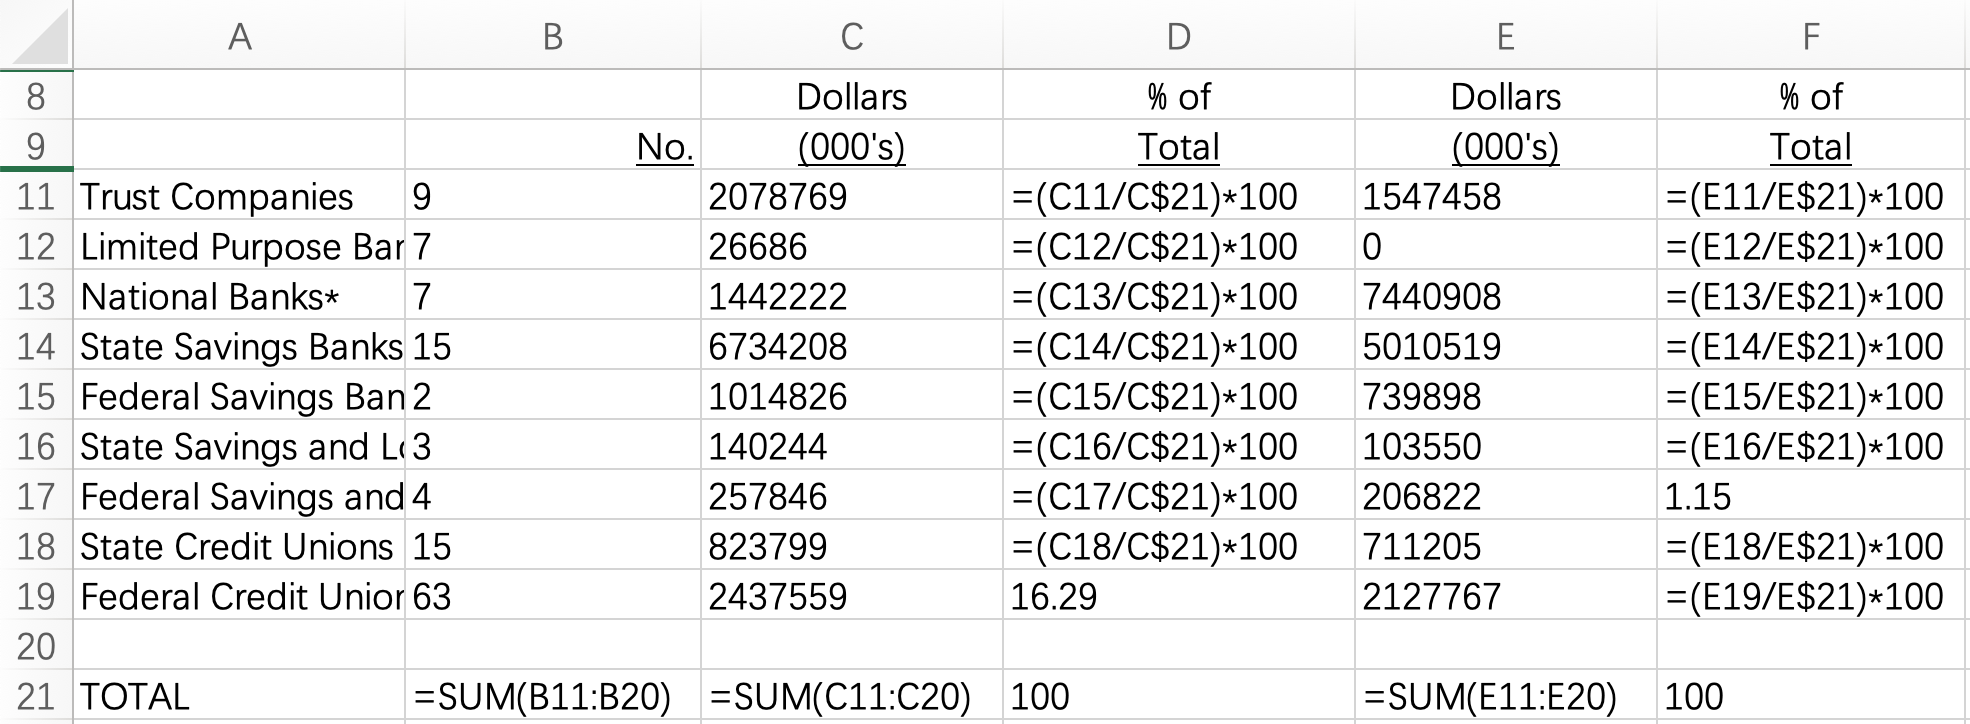
\includegraphics[width=\textwidth]{figure/style-A1.png}
    \caption{截取自EUSES 数据库中的电子表格 summ0602.xls 的工作表summary1201(A1 表示法)}
    \label{figure-A1}
\end{figure}
\begin{figure}[tbp]    
    \centering
    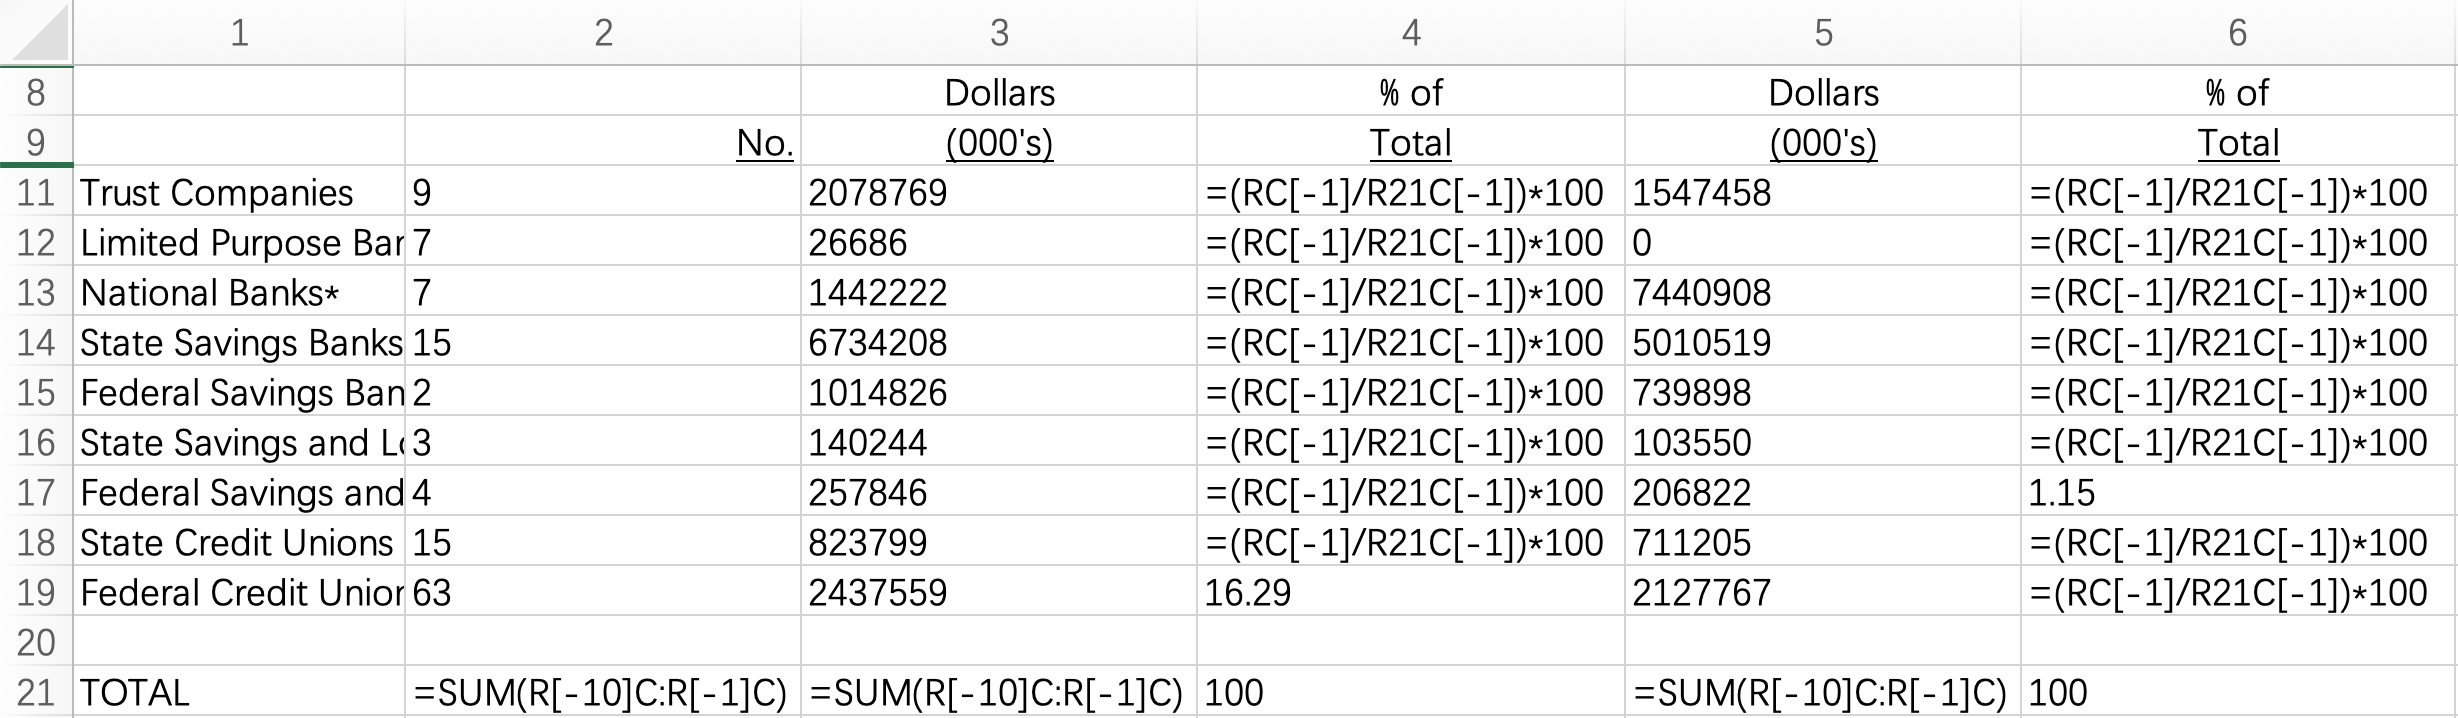
\includegraphics[width=\textwidth]{figure/style-R1C1.png}
    \caption{截取自EUSES 数据库中的电子表格 summ0602.xls 的工作表summary1201(R1C1 表示法)}
    \label{figure-R1C1}
\end{figure}

\begin{definition}
    绝大多数电子表格软件有两种内置的表达公式应用的风格,即\textit{A1表示法} 和 \textit{R1C1表示法} \cite{tan2014bug} ,另一种划分方式是\textit{绝对引用}和\textit{相对引用}。
\end{definition}

绝对引用指向特定的单元格,当它在某个表达式中存在,并且该表达式被复制到其他单元格,仍然引用相同的单元格。
相对引用表示单元格地址在当前单元格和被引用单元格之间的偏移量,当该引用被复制到其他单元格时,偏移量保持不变,但实际引用的单元格地址发生了变化。

在 A1 表示法中,一个在第 $X$ 列第 $y$ 行的单元格在相对引用中表示为 $Xy$(例如$B5$),在绝对引用中表示为 $\$X\$y$(例如$\$B\$5$)。
如图\ref{figure-A1}所示,该电子表格使用的是 A1 表示法,且所有单元格引用都是相对引用。

另一方面,在 R1C1表示法中,一个在当前单元格的下方第$n$行和右侧第$m$列的单元格在相对引用中表示为$R[n]C[m]$(其中,$n$/$m$在$n=0$/$m=0$时可以省略,而一个处在第$n$行,第$m$列的单元格在绝对引用下表示为$RnCm$。
如图\ref{figure-R1C1}所示,该电子表格使用 R1C1表示法,且所有单元格引用都是相对引用。

一个有趣的观察是:含有相似计算模式的公式单元格通常具有语义等价的 R1C1 表示的公式形式。
例如,图\ref{figure-A1}中的单元格 $D11$ 中的公式$(C11/C\$21)*100$ 在 R1C1表示法中是图\ref{figure-R1C1}中的$(RC[-1]/R21C[-1])*100$。
后一个公式表示对两个单元格的值进行除法运算再乘以一百。
第一个值由同一行向左一列的单元格给出,第二个值由第 21 行向左一列的单元格给出。
图\ref{figure-R1C1}也给出了图\ref{figure-A1}中其他所有公式对应的 R1C1 表示结果。
我们不难观察出:其中一些单元格在计算意义上是等价的,或者是相似的。
我们正式利用这一出发点,从中提出特征来讲单元格进行区分,以便形成不同的单元格类,进而检测出每个类中包含的有缺陷的单元格。

在接下来的讨论中,除额外说明,我们假设表达式$exp$和函数$\sigma(exp)$都使用 R1C1表示法。

\section{单元格类}

单元格类的存在通常是为了后续进行单元格缺陷的检测。
类似地,软件测试为了发现代码中的错误,通常要对代码进行静态分析、动态执行,收集抽象或者具体的代码执行记录,通过对记录的分析来寻找代码中的错误根源。
我们对整个工作表进行分类,找出其中包含的不同的单元格类,本质上就是在试图找到该工作表中包含的具有各自计算意义的单元格集合。
进而,在这种单元格集合中,进行细致分析找出潜在的有缺陷的单元格。
这里我们给出单元格类,在本文中的定义:

\begin{definition}
    \textit{单元格类}是单元格的集合,其中每个单元格都具有\textit{相似}的\textit{计算目标}。
\end{definition}

要理解单元格类,需要在各类技术中明确其中的两个关键概念:
\begin{itemize}
    \item \textit{计算目标}的概念:能够直接或者间接表明该单元格的计算目标的特征,都可以用来表征该单元格的计算目标。比如,直接的特征就是该单元格拥有的公式(但该公式可能有缺陷,未必完全准确地反映该单元格的计算目标);间接的特征比如该单元格周围的其他单元格,或者该单元格的表头文字信息等,都可以间接地暗示出该单元格可能拥有的部分计算目标。
    \item \textit{相似}的概念:通常定义相似的方式是量化该单元格在一个单元格集合中,与整个集合中其他单元格的计算目标的相似度。类似地,可以采用比较直接特征和间接特征相似度的方式,来权衡最终两个单元格的相似度。
\end{itemize}
在缺乏终端用户的先验知识的前提下,如何定义计算目标,以及如何量化单元格之间的计算目标相似度,正是各类电子表格缺陷检测技术的设计挑战。

\section{单元格的公式缺陷}

% 这里似乎可以加一句,跟 Chapter 2 里的相关工作相呼应。
在理解单元格类的基础上,我们来进一步解释何为单元格的公式缺陷。
为了解释的方便,我们结合 EUSES 语料库中的一个工作表上的分析结果(如图\ref{figure-sg5}和\ref{figure-sg6})来辅助理解。
这个例子中包含 7 个有缺陷的单元格,其中的 6 个数值单元格极有可能是错误的表达方式。

例如,如果单元格$F17$的值与根据同类里的公式$(RC[-1]/R20C[-1])*100$计算出的值不一致,并且单元格区域$[F11:F19]$的值求和之后并不等于一百,这和单元格$F21$想要得到的计算结果也不一致。
在某些单元格(如$F17$)中的错误可能进一步导致其他单元格的错误(如$F21$)。
通常,有缺陷的单元格中一定存在\textit{替换}导致的异常,通常是用新的子表达式替换了旧的子表达式。
这里,我们根据用于替换的新的子表达式类型来对单元格缺陷进行分类,主要可以归为三类:

\begin{definition}
   \textit{用数值替换的缺陷}:我们把一个单元格用数值(常量)替换一个子表达式(如单元格引用),然而其它的同类单元格并没有这么替换时,这类单元格的缺陷称为用数值替换的缺陷。
\end{definition}
如图\ref{figure-sg6}所示,黄色标记的单元格类包含$[D11:D18]$和$[F11:F18]$这两部分,其中单元格$D16$,$F14$和$F17$都是数值单元格,然而类中的其他单元格都是具有公式$(RC[-1]/R20C[-1])*100$形式的,即这三个有缺陷的单元格用数值替换了整个表达式,进而在后续维护过程中丢失了其本该具有的计算目的,将来可能导致更为严重的错误。

\begin{definition}
    \textit{用不一致的单元格引用替换的缺陷}:类似地,我们把一个单元格用一个错误的单元格或者单元格范围替换一个子表达式,然而其它的同类单元格并没有这么替换时,这类单元格的缺陷称为用不一致的单元格引用替换的缺陷。
\end{definition}

如图\ref{figure-sg6}所示,浅蓝色标记的单元格类包含$[B20:F20]$这五个单元格,其中单元格$F20$引用了一个单元格区域$[F11:F18]$,这和该类中的另外两个公式的引用区域不同,丢失了对单元格$F19$的引用,按照我们对单元格类和单元格计算目标的理解,单元格$F20$包含用不一致的单元格引用替换的缺陷,如果将来某个终端用户在第 19 行填充了相关数据,这会导致$F20$产生错误的计算结果。

\begin{definition}
    \textit{用不一致的操作符/函数替换的缺陷}:类似地,我们把一个单元格用一个错误的操作符/函数替换一个子表达式,然而其它的同类单元格并没有这么替换时,这类单元格的缺陷称为用不一致的操作符/函数替换的缺陷。
\end{definition}
如图\ref{figure-sg6}所示,暗粉色标记的单元格类包含$[B26:F26]$这五个单元格,目前单元格$E26$含有正确且一致的公式形式$SUM(E23:E24)$,但如果用户使用不一致的操作符进行修改,比如改写成$E23 + E24$,那么将来某个终端用户对这个类中的公式进行重构时,可能未必能发现单元格$E26$也属于这个类的一员,进而忽视了对它的修改,可能导致最终的计算结果错误。


上述三类单元格缺陷类型已经在真实商业场景下频繁发现\cite{panko2006facing,powell2008critical}。
学界也存在类似的案例调研,关注电子表格缺陷如何被引入到表格中\cite{dou2014spreadsheet}。
由于缺陷的类型和变体多种多样,普通终端用户在选用电子表格测试技术时,由于并没有预先知道自己的表格中潜在的缺陷类型属于哪一类,并不好针对性的选择特定技术。那么基于学习、单元格聚类的技术因为天生具有对多种缺陷的适应性,能够把上述各种类型的缺陷单元格都尽可能不遗漏地加入到单元格类中,最后再做统一的缺陷检测分析。这对于终端用户来说,是一个更容易接受并采纳的电子表格缺陷检测技术方案。
